%%%%%%%%%%%%%%%%%%%%%%%%%%%%%%%%%%%%%%%%%%%%%%%%
	\begin{frame}
		\frametitle{}
	    \begin{center}
		{ {\Huge 第二章~~三大偏微分方程\\(6学时)}}
	    \end{center}    
	\end{frame}
%%%%%%%%%%%%%%%%%%%%%%%%%%%%%%%%%%%%%%%%%%%%%


\begin{frame}
	\begin{definition}[] 
	偏微分方程(PDE)指未知函数是多元函数的微分方程,
	方程的函数(物理量)多以时间和空间为变量,这些方程的来源和应用通常具有物理学背景。又称为数学物理方程。
	\end{definition}
	对于二阶偏微分方程
	\begin{equation*}
		au_{xx}+2bu_{xy}+cu_{yy}+du_x+eu_y+fu=g
	\end{equation*}
	根据$\Delta=b^2-ac$分为三类:椭圆型($\Delta<0$)、双曲型($\Delta>0$)和 抛物型 ($\Delta=0$),\\
	它们的代表分别是:拉普拉斯(泊松方程)、波动方程、热传导方程
\end{frame}

\begin{frame}
\frametitle{三大偏微分方程}
	\begin{itemize}
	\item  波动方程 
	\begin{equation*}
		u_{tt}=a^2u_{xx}
	\end{equation*}
	\item  热传导方程
	\begin{equation*}
		u_t=a^2 \nabla ^2 u 
	\end{equation*}
	\item  拉普拉斯方程
	\begin{equation*}
		 \nabla ^2 u =0
	\end{equation*}
	\end{itemize}
\end{frame}

%%%%%%%%%%%%%%%%%%%%%%%%%%%%%%%%%%%%%%%%%%%%%
\section{波动方程}
\subsection{方程的建立}
\begin{frame}
	\frametitle{方程的建立}	
	自然界普遍存在各种振动,振动的传播形成波,服从统一的方程。
	\begin{exampleblock} {例1、	求弦振动方程}
	考虑均匀柔软的细弦线,二端固定,受到扰动后在平衡位置作微小运动。分析位移函数 u(x,t)满足的方程。\\
	\begin{tikzpicture}
	%\draw[eaxis] (0,0) -- (8,0) node[below] {$x$};
	%\draw[eaxis] (0,0) -- (0,0.5) node[right] {$y$};
	\draw (0,0) .. controls (2, 1) and (6,1) .. (8,0);
	\filldraw[red] (0,0) circle [radius=1pt];
	\filldraw[red] (8,0) circle [radius=1pt];
	\end{tikzpicture}
	\end{exampleblock} 			
\end{frame}	

\begin{frame}
	\frametitle{}	
	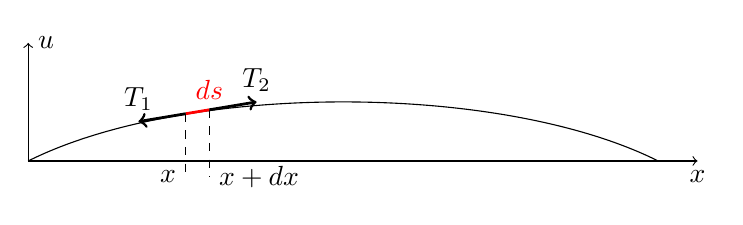
\begin{tikzpicture}
		\draw[->] (0,0) -- (8.5,0) node[below] {$x$};
		\draw[->] (0,0) -- (0,1.5) node[right] {$u$};
		\draw (0,0) .. controls (2, 1) and (6,1) .. (8,0);
		%	\filldraw[red](2,0.6)circle[radius=1pt];
		\draw[dashed] (2,0.6) --(2,-0.2) node[left] {$x$}; 
		%	\filldraw[red](2.3,0.65)circle[radius=1pt];
		\draw[dashed] (2.3,0.65) --(2.3,-0.2) node[right] {$x+dx$}; 
		\draw[red,  line width =1pt] (2,0.6) --(2.3,0.65) node[above] {$ds$};  
		\draw[->, line width =1pt] (2,0.6) --(1.4,0.5) node[above] {$T_1$};  
		\draw[ ->,  line width =1pt] (2.3,0.65) --(2.9,0.75) node[above] {$T_2$};  
	\end{tikzpicture}\\
	\alert{解:} 建立坐标系,  取任意微元ds, 临近拉力$T_1, T_2$:\\
	水平:{ $T_2\cos \alpha _2=T_1\cos \alpha _1=T_0$ }  \\   
	竖直:{$T_2\sin \alpha _2-T_1\sin \alpha _1=ma=\rho ds~ u_{tt} $}   \\   
	有~:{ $T_0(\tan \alpha _2-\tan \alpha _1)=\rho ds ~u_{tt}$ }   \\   
    \hspace{1cm}$T_0[u_x(x+dx,t)-u_x(x,t)]=\rho dx ~u_{tt}$  \\  
	\hspace{1cm}$\displaystyle \frac{T_0}{\rho}\times\frac{u_x(x+dx,t)-u_x(x,t)}{dx}=u_{tt}$ \\
\end{frame}	

\begin{frame}
	\frametitle{}	
	得波动方程:
	\begin{equation*}
		u_{tt}=a^2u_{xx}
	\end{equation*}
	定解条件:\\
	(1) 初始条件 
	$\displaystyle  u(x,t)|_{t=0}= \psi (x) $, 	 $\displaystyle  u_t(x,t)|_{t=0}= \Psi (x) $\\
	(2) 边界条件
	$\displaystyle  u(x,t)|_{x=0}= 0 $, 	 $\displaystyle  u(x,t)|_{x=l}= 0 $\\ 	\vspace{0.3cm} 
	若质点受外力作用, 有:
	\begin{equation*}
		u_{tt}=a^2u_{xx} +f(x,t)
	\end{equation*}
	\begin{block} {Remark}
		波动方程描述了围绕平衡态小幅震荡的规律,它不仅可描述琴弦、鼓膜、耳机的震动,也描述着光波、声波、地震波、引力波,甚至弦论中弦的运动。
	\end{block}
\end{frame}	
%%%%%%%%%%%%%%%%%%%%
\subsection{方程的求解}
\begin{frame}
	\frametitle{方程的求解}	
	\begin{exampleblock} {例2、	求一维波动方程}
	$\displaystyle \begin{cases}
		u_{tt}=a^2u_{xx}\\
		u(x,t)|_{t=0}= \psi (x) ,~~~ u_t(x,t)|_{t=0}= \Psi (x) \\
		u(x,t)|_{x=0}= 0, ~~~  u(x,t)|_{x=l}= 0 
	\end{cases}$ \\	
	\end{exampleblock} %2
	\alert{解:} 	(傅里叶)   设 $\displaystyle  u(x,t)=T(t)X(x) $,代回方程 , 得:
	\begin{equation*}
		 T~^{''}(t)X(x) =a~^2 T(t)X~^{''}(x) 
	\end{equation*}
	 \hspace{1cm} 可分离变量
\end{frame}	

\begin{frame}
	\frametitle{}	
	$ \dfrac{T~^{''}}{a~^2 T}=\dfrac{X~^{''} }{X} =-\lambda $ \\ \vspace{0.3cm}
	转化为两常微分方程 \\ \vspace{0.3cm}
	方程(I):
	$\displaystyle  \begin{cases}
		X~^{''} +\lambda X=0  ~~,~~ 0<x<l\\
		X(0)=0 ~,~X(l)=0
	\end{cases}$ \\	
	方程(II):
	$\displaystyle  \begin{cases}
		T~^{''} +\lambda {a~^2 T}=0 \\
		......
	\end{cases}$ \\	
	\begin{block} {Remark}
		偏微分方程与常微分方程的分离变量法有何不同?
	\end{block}
\end{frame}	

\begin{frame}
	\frametitle{}	
	解方程(I):有特征(辅助)方程, 
	\begin{equation*}
		\mu~^2 +\lambda =0
	\end{equation*}
	根为:
	$\displaystyle  \begin{cases}
		\mu~_1=+\sqrt{-\lambda}\\
		\mu~_2=-\sqrt{-\lambda}
	\end{cases}$ \\		
	分情况讨论:\\
	(1) 相异实根($\lambda < 0$)
	有通解:	{ $\displaystyle 	X=Aexp~^{\sqrt{-\lambda}x} + Bexp~^{-\sqrt{-\lambda}x} $ } \\ 
	分别取$x=0, x=l$, 得定解方程组:\\
	$\left[
	\begin{array}{lll}
		1&1\\
		exp~^{\sqrt{-\lambda}~l} &exp~^{-\sqrt{-\lambda}~l}
	\end{array}
	\right]$
	$\left[
	\begin{array}{ll}
		A\\
		B
	\end{array}
	\right]$
	=$\left[
	\begin{array}{ll}
		0\\
		0
	\end{array}
	\right]$
\end{frame}	

\begin{frame}
\frametitle{}	
	有解条件为:
	$\begin{vmatrix}
		1&1\\
		exp~^{\sqrt{-\lambda}~l} &exp~^{-\sqrt{-\lambda}~l}
	\end{vmatrix}
	= 0$\\
	很明显,这个行列式不等于0, 所以只有零解 (A=0,~B=0)    \\ \vspace{0.3cm}
	(2) 相同实根($\lambda = 0$),\\
	则通解为:	{ $\displaystyle 	X=Ax + B $ } \\ 
	分别取$x=0, x=l$, 得定解方程组:\\
	{$\displaystyle \left\{
	\begin{array}{lll}
		B=0\\
		Al+B=0
	\end{array} \right. $}\\
	也只有零解  \\
\end{frame}	

\begin{frame}
	\frametitle{}	
	(3) 虚根($\lambda >0$),即: $ \mu~_1=i\sqrt{\lambda}~~,~~\mu~_2=-i\sqrt{\lambda}$	\\
	通解为:	{ $\displaystyle 	X=A\cos \sqrt{\lambda}x+ B\sin \sqrt{\lambda}x $ } \\ 
	分别取$x=0, x=l$, 得定解方程组:\\
	$\left[
	\begin{array}{lll}
		1&0\\
		\cos( {\sqrt{\lambda}~l}) &\sin ({\sqrt{\lambda}~l})
	\end{array}
	\right]$
	$\left[
	\begin{array}{ll}
		A\\
		B
	\end{array}
	\right]$
	=$\left[
	\begin{array}{ll}
		0\\
		0
	\end{array}
	\right]$\\ 
	系数行列式要为零\\
	$ \sin ({\sqrt{\lambda}~l})=0$ \\
	$ \sqrt{\lambda}~l=n~\pi  (n=1,2,3,...) $\\ 
	固有值:$\displaystyle  \lambda~_n=\frac{n^2\pi~^2}{l~^2}$ \\ 
	固有解:{\large $\displaystyle  X~_n=B~_n \sin \frac{n\pi~}{l} x=B~_n \sin \omega_n x $}
\end{frame}	

\begin{frame}
	\frametitle{}	
	求解方程II : 	$\displaystyle  T~^{''} +\lambda {a~^2 T}=0 $ \\ 
	代入$\lambda_n$, 得:
	$\displaystyle  T~^{''} +\lambda~_n a~^2 ~T=0 $ \\
	变形成:$\displaystyle  T~^{''} +\omega ~_n ^2 {a~^2 T}=0 $ \\ 
	特征方程有虚根,通解 :\\
	\hspace{3cm}	$\displaystyle 	T~_n=C~_n\cos \omega_n~a~t+ D~_n\sin \omega ~_n~a~t $  \\ 
	原方程的基本解:\\
	$\begin{array}{llll}
		u_n(x,t) &=& T_n(t)X_n(x)\\
		&=& (a_n\cos \omega_nat+ b_n\sin \omega _nat ) \sin \omega_n x\\
		&=&(a_n\cos\frac{ n\pi at}{l}+ b_n\sin \frac{ n\pi at}{l}) \sin \frac{ n\pi x}{l}
	\end{array}$ \\ 
	叠加解 (解函数):\\
 	$\begin{array}{llll}
 		u(x,t) &=&\sum\limits_{n=1}^{\infty } u_n(x,t)\\
 		&=& \sum\limits_{n=1}^{\infty }  (a_n\cos\frac{ n\pi at}{l}+ b_n\sin \frac{ n\pi at}{l}) \sin \frac{ n\pi x}{l}
 	\end{array}$ \\ 
\end{frame}	

\begin{frame}
	\frametitle{}	
	\begin{block} {Remark } 
		叠加解的思考与讨论:
		\begin{itemize}
			\item \textbf {数学理解}: 线性方程解的线性组合,依然是方程的解  
			\item \textbf {物理理解}:It is not complicated. It is just a lot of it. 
			\item \textbf {核心成果}:傅里叶级数与傅里叶变换 
		\end{itemize}
	\end{block}
\end{frame}	

\begin{frame}
	\frametitle{}	
	确定解的系数,\\
	$ \displaystyle u(x,t)= \sum\limits_{n=1}^{\infty }  (a_n\cos\frac{ n\pi at}{l}+ b_n\sin \frac{ n\pi at}{l}) \sin \frac{ n\pi x}{l}$\\
	代入定解条件:\\ 
	(1) $ \displaystyle u(x,0)= \varphi (x)$ ~~=> ~~$\varphi (x)=\sum_{n=1}^{\infty } a_n \sin \frac{ n\pi x}{l}$\\  
	(2) $ \displaystyle u_t(x,0)= \Psi (x)$ ~~=> ~~$\Psi (x)=\sum_{n=1}^{\infty } b_n \frac{ n\pi a}{l} \sin \frac{ n\pi x}{l}$ \\  \vspace{0.3cm}
	由傳里叶变换公式(非对称), 写出系数:\\  
	$ \displaystyle a_n=  \frac{2}{l}\int\limits_{0 }^{l}  \varphi (x) \sin \frac{ n\pi x}{l} dx $\\   
	$ \displaystyle b_n= \frac{l} { n\pi a} \frac{2}{l}\int\limits_{0 }^{l}  \Psi  (x) \sin \frac{ n\pi x}{l} dx =  \frac{2} { n\pi a}  \int\limits_{0 }^{l}  \Psi  (x) \sin \frac{ n\pi x}{l} dx$\\   
\end{frame}	



\subsection{固有函数正交}
\begin{frame}
	\frametitle{固有函数正交性}	
	\begin{exampleblock} {例3、	试证明固有函数的正交性}
		\begin{equation*}
			X~_n= \sin \frac{n\pi~}{l} x  
		\end{equation*}
	\end{exampleblock} 	
	\alert{解:} 固有函数是固有方程的解:\\
	$\begin{array}{llll}
		&X_n ^{''}+\lambda_n X_n=0\\
		&X_m ^{''}+\lambda_m X_m=0
	\end{array}$ \\ 
	用$X_m$乘第一式,$X_n$乘第二式,\\
	$\begin{array}{llll}
		&X_m X_n ^{''}+\lambda_n X_m X_n=0\\
		&X_nX_m ^{''}+\lambda_m X_n X_m=0
	\end{array}$ \\ 
	两式相减:\\
	$\begin{array}{llll}
		& (\lambda_n-\lambda_m) X_n X_m= X_nX_m ^{''}-X_mX_n ^{''} 
	\end{array}$ \\ 
\end{frame}	

\begin{frame}
	\frametitle{}	
	积分:\\
	$ \begin{array}{llll}
		(\lambda_n-\lambda_m) \int\limits_{0 }^{l}  X_n X_m dx &= & \int\limits_{0 }^{l}  [X_nX_m ^{''}-X_mX_n ^{''} ] dx\\   \vspace{0.3cm}
		&=&  [X_nX_m ^{'}-X_mX_n ^{'} ]_0 ^{l} - \int\limits_{0 }^{l}  [X_n ^{'} X_m ^{'}-X_m ^{'} X_n ^{'} ] dx \\   
	\end{array}$ \\
	等式右边的两项分别为零,有\\
	$ \begin{array}{llll}
		(\lambda_n-\lambda_m) \int\limits_{0 }^{l}  X_n X_m dx=0 \\   
	\end{array}$ \\
	$ \begin{array}{llll}
		\int\limits_{0 }^{l}  X_n X_m dx=0 ~~,~~~ (n\ne m)\\   
	\end{array}$ 
\end{frame}	

\begin{frame}
	\frametitle{}	
	当$n= m \ne 0$时, \\   
	$ \begin{array}{llll}
		\int\limits_{0 }^{l}  X_n X_m dx&= \int\limits_{0 }^{l}  X_n X_n dx \\
		&= \int\limits_{0 }^{l}   \sin ^2  \frac{n\pi~}{l} x dx \\
		&=  \dfrac{l}{2}  
	\end{array}$ \\
	归一化系数:
	\begin{equation*}
		A=\sqrt{\frac{l}{2}}
	\end{equation*}
\end{frame}	

\begin{frame}
	\frametitle{求解实例}	
	\begin{exampleblock} {例4、	求解零初边值问题}
	$\displaystyle  \begin{cases}
		u_{tt} =u_{xx} ~~,~~ 0<x<1, t>0\\
		u(0,t) =u(1,t)=0 \\
		u(x,0) =\sin \pi x, u_t (x,0)=0 
	\end{cases}$ \\	
	\end{exampleblock} 	
	\alert{解:}
	固有值:$\displaystyle  \lambda~_n=\dfrac{n^2\pi~^2}{l~^2 }= n^2\pi~^2 $ \\ 
	固有函数:$\displaystyle  X~_n=B~_n \sin \dfrac{n\pi~}{l} x=B~_n \sin n\pi x $\\
	解函数:
	$\begin{array}{llll}
		u(x,t)&=& \sum\limits_{n=1}^{\infty }  (a_n\cos\dfrac{ n\pi at}{l}+ b_n\sin \dfrac{ n\pi at}{l}) \sin \dfrac{ n\pi x}{l}\\
		&= &\sum\limits_{n=1}^{\infty }  (a_n\cos n\pi t+ b_n\sin n\pi t ) \sin n\pi x \\
	\end{array}$ \\ 
\end{frame}	

\begin{frame}
	\frametitle{}	
	$\begin{array}{lllllllll}
		a_n&=  \dfrac{2}{l} \int\limits_{0 }^{l}  \varphi (x) \sin \dfrac{ n\pi x}{l} dx \\
		&= 2 \int\limits_{0 }^{1}  \sin(\pi x) \sin n\pi x dx \\
		&= 2 \int\limits_{0 }^{1}  \sin(\pi x) \sin \pi x dx  \\
		&=1~~  (n=1)   \\
		b_n&= \dfrac{2} { n\pi a} \int\limits_{0 }^{l}  \Psi  (x) \sin \dfrac{ n\pi x}{l} dx  \\
		&= \dfrac{2} { n\pi} \int\limits_{0 }^{1}  0  \sin n\pi x dx  =0\\
	\end{array}$ \\ 
	解函数:$\displaystyle  u(x,t) = \cos(\pi t) \sin(\pi x)   $\\
\end{frame}	

\begin{frame}
	\frametitle{作业:}	
	求解波动方程初边值问题
	$\begin{array}{lllllllll}
	1. & \begin{cases}
		u_{tt} =a^2u_{xx} ~~,~~ 0<x<l, t>0\\
		u(0,t) =u(l,t)=0 \\
		u(x,0) =sin \dfrac{\pi x}{l} ,  u_t (x,0)=\sin \pi x 
	\end{cases}\\	
	2. &\begin{cases}
		u_{tt} =a^2u_{xx} ~~,~~ 0<x<l, t>0\\
		u(0,t) =u(l,t)=0 \\
		u(x,0) =3sin \dfrac{3\pi x}{2l} +6\sin(\dfrac{5\pi x}{2l}),  u_t (x,0)=0
	\end{cases} \\	
	3. &\begin{cases}
		u_{tt} =u_{xx} ~~,~~ 0<x<1, t>0\\
		u(0,t) =u(l,t)=0  \\
		u(x,0) =\sin 2\pi x ,  u_t (x,0)=x (1-x) 
	\end{cases} \\	
	\end{array}$ \\ 	
\end{frame}	


%%%%%%%%%%%%%%%%%%%%%%%%%%%%%%%%%%%%%%%%%%%%%
\section{热传导方程}
\subsection{方程的建立}
\begin{frame}
	\frametitle{}	
	\begin{exampleblock} {例1、建立热传导方程}
		实验发现,热量总是从温度高的地方传向温度低的地方,服从傅里叶热传导定律:
		\begin{equation*}
			q=-k\nabla u
		\end{equation*}
		式中,q是热流强度 (定义为单位时间通过单位横截面积的热量); k 是材料的导热系数 ;$\nabla $ 是梯度算子~$(\frac{\partial }{\partial x} +\frac{\partial }{\partial y} +\frac{\partial }{\partial z})$。\\
		对于介质中任意小体积($d\tau $),试建立温度函数u(x,y,z,t)所满足的方程 。\\
		~~~\hspace*{\fill} \\	
	\end{exampleblock}
\end{frame}	

\begin{frame}
	\frametitle{}
	~~~\hspace*{\fill} \\	
	~~~\hspace*{\fill} \\	
	%\usetikzlibrary {3d} 
	\tikzset{math3d/.style={x={(-0.353cm,-0.353cm)},z={(0cm,1cm)},y={(1cm,0cm)}}}
	\opencutright 
	\def\windowpagestuff{\flushright 
	\begin{tikzpicture}[math3d]
			\def\k{1.4}
			\draw [ ->] (-\k,-\k,-\k) --  (\k,-\k,-\k)  node[below] {$z$};
			\draw [ ->]  (-\k,-\k,-\k) -- (-\k, \k,-\k)   node[above] {$x$};
			\draw [ ->]  (-\k,-\k,-\k) -- (-\k,-\k, \k)    node[left] {$y$};
			\def\a{0.5}
			\def\b{0.5}
			\def\c{0.5}
			\coordinate (A01) at ( \a, \b, \c);
			\coordinate (A02) at ( \a,-\b, \c);
			\coordinate (A03) at (-\a,-\b, \c);
			\coordinate (A04) at (-\a, \b, \c);
			\coordinate (A05) at ( \a, \b,-\c);
			\coordinate (A06) at ( \a,-\b,-\c);
			\coordinate (A07) at (-\a,-\b,-\c);
			\coordinate (A08) at (-\a, \b,-\c);
			\draw(A01)--(A02)--(A03)--(A04)--cycle;
			\draw(A06)--(A05)--(A08);
			\draw[dash dot](A06)--(A07)--(A08);
			\draw(A01)--(A05)(A02)--(A06)(A04)--(A08);
			\draw[dash dot](A03)--(A07);
			\draw[line width =1pt]  (-\k,-1,-\k) node[below] {$x$}-- (-\k, 0.0,-\k)  node[below] {$x+dx$}; 
	\end{tikzpicture}}	
	\begin{cutout} {0}{7cm}{2cm}{6}
		\alert{解:}
		傅里叶热传导定律有分量形式 \\
		$~~~~~~q_{x_i}=-k \dfrac{\partial }{\partial x_{i}} u$ \\
		考虑单位时间 x 方向的净流入:\\
		~~~\hspace*{\fill} \\	
		$\displaystyle- (q_x|_{x+dx}-q_x|_x)dydz$ \\
		$\begin{array}{llll}
			&=-\dfrac{\partial q_x }{\partial x}  dxdydz\\
			&= \dfrac{\partial }{\partial x} (k\dfrac{\partial u}{\partial x})dxdydz \\
		\end{array}$ \\   
		总的净流入为:
		\begin{equation*}
			[\frac{\partial }{\partial x} (k_x\frac{\partial u}{\partial x}) + \frac{\partial }{\partial y} (k_y\frac{\partial u}{\partial y}) + \frac{\partial }{\partial z} (k_z\frac{\partial u}{\partial z}) ]dxdydz 
		\end{equation*}
	\end{cutout} 	
\end{frame}	

\begin{frame}
	\frametitle{}	
	流入的热量导致介质温度发生变化(热量守恒定律)\\
	\begin{equation*}
		c \rho \frac{\partial u}{\partial t}dxdydz=[\frac{\partial }{\partial x} (k_x\frac{\partial u}{\partial x}) + \frac{\partial }{\partial y} (k_y\frac{\partial u}{\partial y}) + \frac{\partial }{\partial z} (k_z\frac{\partial u}{\partial z}) ]dxdydz 
	\end{equation*}
	其中c是比热,$\rho$ 是质量密度。 对于各向同性介质:
	\begin{equation*}
		c \rho \frac{\partial u }{\partial t}=k[\frac{\partial }{\partial x} (\frac{\partial u}{\partial x}) + \frac{\partial }{\partial y} (\frac{\partial u}{\partial y}) + \frac{\partial }{\partial z} (\frac{\partial u}{\partial z}) ]	
	\end{equation*}
	\begin{equation*}
		\frac{\partial u }{\partial t}=\frac{k}{c\rho}[\frac{\partial }{\partial x} (\frac{\partial u}{\partial x}) + \frac{\partial }{\partial y} (\frac{\partial u}{\partial y}) + \frac{\partial }{\partial z} (\frac{\partial u}{\partial z}) ]	
	\end{equation*}
	\begin{equation*}
		u_t=a^2 [u_{xx}   +u_{yy}  +u_{zz}] 
	\end{equation*}
	\begin{equation*}
		u_t=a^2 \nabla ^2 u = a^2 \triangle u	
	\end{equation*}
\end{frame}	

\begin{frame}
	\frametitle{}	
	对于一维导线:
	{ $\displaystyle u_t= a^2 u_{xx}$ }  \\ 
	如果有热源F(x,y,z,t),令 $f=\dfrac{F}{c\rho}$:	{$\displaystyle u_t= a^2 u_{xx}+f$ }  \\
	如果时间足够长,温度应不再随时间变化 ($u_t =0$), \\ 
	得无源Laplace 方程: { $\displaystyle   \nabla ^2 u =0$ }  \\ 
	和有源Poisson 方程: { $\displaystyle   \nabla ^2 u =-f$ }  \\ 
	\begin{block}{Remark}
		传导方程描述了热、电、声、磁、光等传输的基本规律,也称输运方程
	\end{block}
\end{frame}	

\subsection{方程的求解}
\begin{frame}
	\frametitle{方程的求解}	
	\begin{exampleblock} {例2、求解热传导方程}
	对于有限长导线,求解一维热传导方程初边值问题 \\
	$\displaystyle \begin{cases}
		u_{t}=a^2u_{xx} ,~~~~ (0<x<l, t>0)\\
		u(x,t)|_{t=0}= \psi (x)  \\
		u(x,t)|_{x=0}= 0, ~~~  u(x,t)|_{x=l}= 0 
	\end{cases}$ \\
	\end{exampleblock}
	\alert{解:} 方程可分离变量,
	设 $\displaystyle  u(x,t)=T(t)X(x) $,代回方程 \\
	\begin{equation*}
		T~^{'}(t)X(x) =a~^2 T(t)X~^{''}(x) 
	\end{equation*}
	\begin{equation*}
		\frac{T~^{'}}{a~^2 T}=\frac{X~^{''} }{X} =-\lambda 
	\end{equation*}
\end{frame}	

\begin{frame}
	\frametitle{}	
	即偏微分方程转化为两常微分方程 \\
	方程(I):\\
	$\displaystyle  \begin{cases}
		X~^{''} +\lambda X=0  ~~,~~ 0<x<l\\
		X(0)=0 ~,~X(l)=0
	\end{cases}$ \\	
	方程(II):\\
	$\displaystyle  \begin{cases}
		T~^{'} +\lambda {a~^2 T}=0 \\
		......
	\end{cases}$ \\	
	~~~\hspace*{\fill} \\	
	方程(I)是固有值问题,有解:\\
	固有值:$\displaystyle  \lambda~_n=\frac{n^2\pi~^2}{l~^2}$ \\ 
	固有函数:{$\displaystyle  X~_n= \sin \frac{n\pi~}{l} x$}\\
\end{frame}	

\begin{frame}
	\frametitle{}	
	解方程II : 	$\displaystyle  T~^{'} +\lambda {a~^2 T}=0 $ \\ 
	代入$\lambda_n$, 得:
	$\displaystyle  T~^{'} +\lambda~_n a~^2 ~T=0 $ \\
	变形成:$\displaystyle  T~^{'} + rT=0 $ \\ 
	这是衰减数学模型,有公式:
	\begin{equation*}
		T= Bexp(-rt)
	\end{equation*}
	通解 :$\displaystyle T_n=B_n  \exp(-(\dfrac{n\pi a}{l})^2 t)$ \\  
	原方程的基本解为:\\ \vspace{0.3cm}
	$\begin{array}{llll}
		u_n(x,t) &= T_n(t)X_n(x)\\
		&= B_n  \exp(-(\dfrac{n\pi a}{l})^2 t) \sin \dfrac{n\pi~}{l} x \\
	\end{array}$ \\ 
\end{frame}	

\begin{frame}
	\frametitle{}	
	代入定解条件:\\ 
	$ \displaystyle u(x,0)= \psi(x)$ ~~=> \\
	$\psi (x)=\sum\limits_{n=1}^{\infty } B_n \sin \dfrac{ n\pi }{l} x$\\  
	由傳里叶变换公式(非对称),得系数:\\  
	$ \displaystyle B_n=  \dfrac{2}{l}\int\limits_{0 }^{l}  \psi (x) \sin \dfrac{ n\pi }{l} x dx , ~~~ (n=1,2,3,...) $\\   
\end{frame}	

\begin{frame}
	\begin{exampleblock} {例3、求解热传导方程}
	对于有限长的导线,求解如下一维热传导方程 
	$\displaystyle \begin{cases}
		u_{t} =u_{xx} ,~~ 0<x<L, ~~t>0\\
		u(0,t) =0, ~~u(L,t)=0 \\
		u(x,0) =x(L-x)
	\end{cases}$ \\
	\end{exampleblock}
	\alert{解:} 
	零边界条件确定的固有值和固有函数:\\
	固有值:$\displaystyle  \lambda~_n=\dfrac{n^2\pi~^2}{l~^2 }= (\dfrac{n\pi }{L}) ^2$ \\ 
	固有函数:$\displaystyle  X~_n=\sin \dfrac{n\pi~}{l} x=\sin \dfrac{n\pi~}{L} x $\\	
\end{frame}	

\begin{frame}
	\frametitle{}	
	解函数:\\ 
	$\displaystyle \begin{array}{llll}
		u(x,t)&=\sum\limits_{n=1}^{\infty } B_n  \exp(-(\dfrac{n\pi a}{l})^2 t) \sin \dfrac{n\pi~}{l} x\\
		&= \sum\limits_{n=1}^{\infty } B_n  \exp(-(\dfrac{n\pi a}{L})^2 t) \sin \dfrac{n\pi~}{L} x \\
	\end{array}$ \\ 
	$\displaystyle \begin{array}{lllllllll}
		B_n&= \dfrac{2}{l}\int_{0 }^{l}  \psi (x) \sin \dfrac{ n\pi }{l} x dx  \\
		&= \dfrac{2}{L}\int_{0 }^{L}  x(L-x) \sin \dfrac{ n\pi }{L} x dx  \\
		&=\dfrac{2}{L} \times2\times (\dfrac{L2}{n\pi})^3  [1-\cos n \pi ]  \\
		&= 4 \dfrac{L^2}{(n\pi)^3}[1-(-1)^n ]  \\
	\end{array}$ \\ 
	解函数:$\displaystyle  u(x,t) =  (\dfrac{4L^2}{\pi ^3}) \sum_{n=1}^{\infty} \dfrac{1}{n^3} [1-(-1)^n ]  \exp(-(\dfrac{n\pi a}{L})^2 t) \sin \dfrac{n\pi~}{L} x  $\\	
\end{frame}	

\subsection{三类边界条件}
\begin{frame}
	\frametitle{固有值问题II}
	\begin{exampleblock} {例4、求解第二类边界条件热传导方程}
	$\displaystyle  \begin{cases}
		u_{t} =u_{xx} ~~,~~ 0<x<l, t>0\\
		u_x (0,t) =0, u_x (l,t)=0 \\
		u(x,0) =\psi(x)
	\end{cases}$ \\	
	\end{exampleblock}
	\alert{解:} 	
	分离变量后,偏微分方程可转化为 \\
	方程(I):\\
	$\displaystyle  \begin{cases}
		X~^{''} +\lambda X=0  ~~,~~ 0<x<l\\
		X'(0)=0 ~,~X' (l)=0
	\end{cases}$ \\	
	方程(II):\\
	$\displaystyle  \begin{cases}
		T~^{'} +\lambda {a~^2 T}=0 \\
		......
	\end{cases}$ \\	
\end{frame}	

\begin{frame}
	\frametitle{}
	注意到方程(I)是导数边界条件(二类边界条件),不是原固值问题。\\
	先求方程(I):根据以前的讨论,只有在$\lambda >0 $ 即特征方程有虚根时,方程才有非零解。\\
	通解为:
	\begin{equation*}
		X=A\cos \sqrt{\lambda} x + B \sin \sqrt{\lambda} x
	\end{equation*}
	求导:
	\begin{equation*}
		X' (x)=\sqrt{\lambda} [-A\sin \sqrt{\lambda} x + B \cos \sqrt{\lambda} x]
	\end{equation*}
	代入导数边界条件(分别取$x=0, x=l$),得方程组 \\
	$\left[
	\begin{array}{lll}
		0&1\\
		-\sin( {\sqrt{\lambda}~l}) &\cos ({\sqrt{\lambda}~l})
	\end{array}
	\right]$
	$\left[
	\begin{array}{ll}
		A\\
		B
	\end{array}
	\right]$
	=$\left[
	\begin{array}{ll}
		0\\
		0
	\end{array}
	\right]$\\ 	
\end{frame}	

\begin{frame}
	\frametitle{}
	系数行列式为零,得$ \sin\sqrt{\lambda}~l =0$\\
	固有值:
	\begin{equation*}
		\lambda_n =(\frac{n\pi}{l})^2 ~~,~~ (n=0,1,2,......)
	\end{equation*}
	代回方程组,得待定系数:$ [A, B] ^T =[1, 0] ^T$\\
	固有函数:
	\begin{equation*}
		X_n=\cos \frac{n\pi}{l} x~,~~~  (n=\textcolor{red}{0},1,2,......)
	\end{equation*}
	级数解:
	\begin{equation*}
		u(x,t)=\sum\limits_{n=0}^{\infty } B_n  \exp(-(\frac{n\pi a}{l})^2 t) \cos \frac{n\pi~}{l} x
	\end{equation*}
	系数:
	$\displaystyle  \begin{cases}
		B_0&= \dfrac{1}{l} \int_{0}^{l} \psi(x) dx \\
		B_n&= \dfrac{2}{l} \int_{0}^{l} \psi(x) \cos \dfrac{n\pi}{l} xdx ,~~ (n=1,2,......)
	\end{cases}$ \\	
\end{frame}	

\begin{frame}
	\frametitle{}
	级数解:
	\begin{equation*}
		u(x,t)=\frac{B_0 }{2}+ \sum\limits_{n=1}^{\infty } B_n  \exp(-(\frac{n\pi a}{l})^2 t) \cos \frac{n\pi~}{l} x
	\end{equation*}	
	\begin{block} {Remark }
		导致边界条件导致:
		\begin{itemize}
			\item  固有函数:$X~_n=\sin \dfrac{n\pi~}{l} x$ $\to$ 	$X_n=\cos \dfrac{n\pi}{l} x$
			\item 	存在n=0 项 :$\cos \frac{n\pi}{l} = \cos \frac{0\pi}{l} =1$
		\end{itemize}
	\end{block}
\end{frame}	

\begin{frame}
	\frametitle{}
	\begin{exampleblock} {例5、求解如下初边值问题}
	$\displaystyle  \begin{cases}
		u_{t} =u_{xx} ~~,~~ 0<x<\pi, t>0\\
		u_x (0,t) =0, u_x (l,t)=0 \\
		u(x,0) =x^2 (\pi-x)^2
	\end{cases}$ \\	
	\end{exampleblock}
	\alert{解:} 	
	这是导数边界条件,确定的固有值和固有函数为:\\
	固有值:$\displaystyle  \lambda~_n=\dfrac{n^2\pi~^2}{l~^2 }= (\dfrac{n\pi }{\pi}) ^2 = n^2$ \\ 
	固有函数:$\displaystyle  X~_n=\cos \dfrac{n\pi~}{l} x=\cos nx $\\
	解函数:\\ 
	$\displaystyle \begin{array}{llll}
		u(x,t)&=  \sum\limits_{n=0}^{\infty } B_n  \exp(-(\dfrac{n\pi a}{l})^2 t) \cos \dfrac{n\pi~}{l} x\\
	\end{array}$ \\ 	
\end{frame}	

\begin{frame}
	\frametitle{}
	$\displaystyle \begin{array}{lllllllll}
		B_0&=\dfrac{2}{l} \int_{0}^{l} \psi(x) dx   \\
		&= \dfrac{2}{\pi} \int_{0}^{\pi}  x^2 (\pi-x)^2 dx  \\
		&=\dfrac{\pi ^4}{15}\\
		B_n&=\dfrac{2}{l} \int_{0}^{l} \psi(x) \cos \dfrac{n\pi}{l} xdx \\
		&= \dfrac{2}{\pi} \int_{0}^{\pi}   x^2 (\pi-x)^2   \cos nx dx \\
		&= \dfrac{2}{\pi} \times (-\dfrac{12 \pi}{n^4})  [\cos n\pi +1 ] \\
		&= -\dfrac{24}{n^4} [ (-1)^n +1 ] \\
	\end{array}$ \\ 
	解函数:$\displaystyle  u(x,t) =  \frac{\pi ^4}{30} -24 \sum_{n=1}^{\infty } \frac{(-1)^n +1 }{n^4}  \exp(-(na)^2 t) \cos n x$\\
\end{frame}	

\begin{frame}
	\frametitle{}
	\begin{alertblock}{直接计算$n_0$项}
		$u(x,t)=  \sum\limits_{n=0}^{\infty } B_n  \exp(-(\dfrac{n\pi a}{l})^2 t) \cos \dfrac{n\pi~}{l} x$\\
		代入初值条件: $x^2 (\pi-x)^2=  \sum\limits_{n=0}^{\infty } B_n  \cos \dfrac{n\pi~}{l} x$\\
		取出第0项: $x^2 (\pi-x)^2=  B_0  \cos \dfrac{0\pi~}{l} x $\\
		积分: $\int\limits_{0} ^ \pi  x^2 (\pi-x)^2 dx = \int\limits_{0} ^ \pi   B_0  dx $\\
		\hspace{1cm}  $\dfrac{1}{6}  \int\limits_{0} ^ \pi  (\pi-x)^4 dx = B_0 \pi$\\
		\hspace{1cm}  $B_0 = \dfrac{1}{6\pi}  \int\limits_{0} ^ \pi  (\pi-x)^4 dx = \dfrac{\pi ^4}{30} $
   \end{alertblock}
\end{frame}	

\begin{frame}
	\begin{alertblock}{定积分计算细节}
		令 $\psi (x) = x^2 (\pi-x)^2$ ,求导:\\
		$\displaystyle \begin{array}{lllllllll}
			\psi ' (x) &=  2x(2x - \pi )(x - \pi ) \\
			\psi '' (x) &=  2\pi ^2 -12\pi x+12x^2 \\
			\psi ''' (x) &=  24x -12 \pi \\
			\psi^{(4)} (x) &=  24  \\
		\end{array}$ \\ 
		令 $\nu^{(4)} (x) = \cos nx$ , 则:\\
		$\displaystyle \begin{array}{lllllllll}
			\nu ''' (x) &= \dfrac{1}{n} \sin nx \\
			\nu '' (x) &= -\dfrac{1}{n^2} \cos nx \\
			\nu ' (x) &= -\dfrac{1}{n^3} \sin nx \\
			\nu (x) &= \dfrac{1}{n^4} \cos nx \\
		\end{array}$ \\ 
	\end{alertblock}
\end{frame}	

\begin{frame}
	得:
	\begin{equation*}
		\int_{0}^{\pi}  \psi^{(4)} (x)  \nu (x)  dx = \frac{24}{n^4} \int_{0}^{\pi}  \cos nx dx =0
	\end{equation*}
	应用分部积分公式,有 \\
	$\displaystyle \begin{array}{lllllllll}
		&\int\limits_{0}^{\pi}  \psi (x) \nu^{(4)} (x)  dx \\
		&= [ \psi \nu''' - \psi' \nu'' + \psi'' \nu' -\psi''' \nu ]|_0 ^\pi +	\int\limits_{0}^{\pi}  \psi^{(4)} (x)  \nu (x)  dx  \\
		&=  [ \psi \nu''' - \psi' \nu'' + \psi'' \nu' -\psi''' \nu ]|_0 ^\pi 
	\end{array}$ \\ 
	所以:
	\begin{equation*}
		\int\limits_{0}^{\pi}  \psi (x) \nu^{(4)} (x)  dx = [-\psi''' \nu ]|_0 ^\pi =  -\dfrac{12 \pi}{n^4}  [\cos n\pi +1 ]
	\end{equation*}
\end{frame}	

\begin{frame}
	\frametitle{第三类边界条件}
	求第三类边界条件的固有值问题\\
	$\begin{array}{lllllllll}
	III & \begin{cases}
			X'' (x)  + \lambda X =0   ~~,~~ 0<x<L\\
			X' (0) =0, X (L) =0
	\end{cases}\\	
	& \begin{cases}
		\lambda_n=\dfrac{(2n+1)^2 \pi ^2}{4l^2}\\
		X_n(x) = \cos \sqrt{\lambda} x
	\end{cases}\\	
	IV&\begin{cases}
		X'' (x)  + \lambda X =0   ~~,~~ 0<x<L\\
		X (0) =0, X' (L) =0
	\end{cases} \\	
	& \begin{cases}
		\lambda_n=\dfrac{(2n+1)^2 \pi ^2}{4l^2}\\
		X_n(x) = \sin \sqrt{\lambda} x
    \end{cases}\\	
	\end{array}$ \\ 
\end{frame}	

\begin{frame}
	\frametitle{作业-1}
	1、求解热传导方程初边值问题\\
	$\begin{array}{lllllllll}
		&\begin{cases}
			u_{t} =a^2u_{xx} ~~,~~ 0<x<l, t>0\\
			u(0,t) =u(l,t)=0 \\
			u(x,0) =x (l-x)
		\end{cases}\\	
		&\begin{cases}
			u_{t} =a^2u_{xx} ~~,~~ 0<x<l, t>0\\
			u_x(0,t) =u_x(l,t)=0 \\
			u(x,0) =x(l-x/2)
		\end{cases} \\	
	\end{array}$ \\ 
	2、求第三类边界条件固有值问题,并求固有函数的正交性\\
	$\begin{array}{lllllllll}
		& \begin{cases}
			X'' (x)  + \lambda X =0   ~~,~~ 0<x<L\\
			X' (0) =0, X (L) =0
		\end{cases}\\	
		&\begin{cases}
			X'' (x)  + \lambda X =0   ~~,~~ 0<x<L\\
			X (0) =0, X' (L) =0
		\end{cases} \\	
	\end{array}$ \\ 	
\end{frame}	

\begin{frame}
	\frametitle{作业-2}
	3. 什么是固有值?有何用处?
	\\
	4. 什么是固有函数?与固有值有何关系? 
	\\
	5. 分离变量法的数学思想是什么?
	\\
	6. 什么是叠加原理?与分离变量法有何关系
	\\
	7. 正交性是什么意思?有何用处?
	\\
	8. 较复杂的分部积分法怎么用?	
\end{frame}	


%%%%%%%%%%%%%%%%%%%%%%%%%%%%%%%%%%%%%%%%%%%%%
\section{拉普拉斯方程}
\subsection{方程的建立}
\begin{frame}
	\frametitle{方程的建立}
	\begin{exampleblock} {例1、建立拉普拉斯方程}
		对于位于原点的质量为M的质点,试建立其引力势函数
		u(x,y,z,t) 所满足的方程 .
	\end{exampleblock}
	%%\usetikzlibrary {3d} 
	\tikzset{math3d/.style={x={(-0.353cm,-0.353cm)},z={(0cm,1cm)},y={(1cm,0cm)}}}
	\opencutright 
	\def\windowpagestuff{\flushright 
	\begin{tikzpicture}
		\def\k{1.5}
		\draw [ ->] (0,0,0) --  (0,0,2.5)  node[below] {$z$};
		\draw [ ->]  (0,0,0) -- (\k, 0,0)   node[right] {$x$};
		\draw [ ->]  (0,0,0) -- (0,\k, 0)    node[right] {$y$};
		\fill[black!100] (0,0,0) node[right]{$M$} circle(0.8ex);
		\begin{scope}[canvas is zy plane at x=0] \draw (0,0) circle (1cm);
			\draw (-1,0) -- (1,0) (0,-1) -- (0,1);
		\end{scope};
		\begin{scope}[canvas is zx plane at y=0] \draw (0,0) circle (1cm);
			\draw (-1,0) -- (1,0) (0,-1) -- (0,1);
		\end{scope};
		\begin{scope}[canvas is xy plane at z=0] \draw (0,0) circle (1cm);
			\draw (-1,0) -- (1,0) (0,-1) -- (0,1);
		\end{scope};
	\end{tikzpicture}	}
	~~~\hspace*{\fill} \\	
	~~~\hspace*{\fill} \\	
	\begin{cutout} {0}{6cm}{0pt}{6}
		\alert{ 解:}	建立如图坐标系,\\
		在空间任一点(x,y,z)放置试验质点m\\
 		m感受的力为:\\
		{$ \overrightarrow{F} =-G\dfrac{Mm}{r^3} \overrightarrow {r} $ }  ~~,~~ $r=\sqrt{x^2+y^2+z^2}$\\ 
		M激发的引力场强为 \\
		{ $ \overrightarrow{A} =\dfrac{GM}{r^3} \overrightarrow{r} $ }\\
	\end{cutout}
\end{frame}	

\begin{frame}
	\frametitle{}
	取无穷远处场强为零,则引力势为\\
	$\displaystyle  u = -\int_{r}^{\infty} \overrightarrow{A}\cdot d \overrightarrow{r} =- \int_{r}^{\infty} \frac{GM}{r^2} dr =- \frac{GM}{r} $ \\
	即有: $\overrightarrow{A} =-\nabla u$ \\
	封闭球面S内的质量通量为 \\
	$\displaystyle \oint_{S} \overrightarrow{A} \cdot d \overrightarrow{S} = \frac{GM}{r^2} 4\pi r^2 =\int  4\pi G  \rho d\tau$  \\
	由高斯定理可知:\\
	$ \displaystyle \oint_{S} \overrightarrow{A} \cdot d \overrightarrow{S} =\int  \nabla \cdot \overrightarrow{A} d\tau $\\
	因此: 
	\begin{equation*}
		\nabla \cdot \overrightarrow{A} = 4\pi G \rho
	\end{equation*}
	由于 $\nabla \cdot \overrightarrow{A} = \nabla \cdot \left(-\nabla u\right)= -\nabla ^2 u$ \\
	得泊松方程:
	\begin{equation*}
		\nabla ^2 u= -4\pi G \rho
	\end{equation*}	
\end{frame}	

\begin{frame}
	\frametitle{}
	对于无源区域,得拉普拉斯方程
	\begin{equation*}
		\nabla ^2  u =0 
	\end{equation*}
	定义拉普拉斯算子:
	\begin{equation*}
		\triangle  = \nabla ^2 = \frac{\partial ^2}{\partial x^2} +\frac{\partial^2 }{\partial y^2} +\frac{\partial^2  }{\partial z^2}	
	\end{equation*}
	拉普拉斯方程为:
	\begin{equation*}
		\triangle   u =0 
	\end{equation*}
	\begin{block}{Remark}
		拉普拉斯方程和泊松方程是描述各种势场的基本方程。
	\end{block}
\end{frame}	


\subsection{方程的求解}
\begin{frame}
	\frametitle{}
	\begin{exampleblock} {例2、求解矩形区域拉普拉斯方程}
		$\displaystyle \begin{cases}
			u_{xx} +u_{yy} =0 ,~~~~ (0<x<a, 0<y<b)\\
			u(x,0)= f_1 (x) ,  u(x,b)= f_2 (x) \\
			u(0,y)= g_1 (y) ,  u(a,y)= g_2 (y) 
		\end{cases}$ \\
	\end{exampleblock}	
	\alert{ 解:}	这是第一类边界条件,但不是零边界条件,可转化为 \\
	$\displaystyle (A) \begin{cases}
		u_{xx} +u_{yy} =0 ,~~~~ (0<x<a, 0<y<b)\\
		u(x,0)= 0,  u(x,b)= 0 \\
		u(0,y)= g_1 (y) ,  u(a,y)= g_2 (y) 
	\end{cases}$ \\
	$\displaystyle (B) \begin{cases}
		u_{xx} +u_{yy} =0 ,~~~~ (0<x<a, 0<y<b)\\
		u(x,0)= f_1 (x) ,  u(x,b)= f_2 (x) \\
		u(0,y)= 0,  u(a,y)= 0 
	\end{cases}$ \\
	当然,还可以进一步分解成四个边值问题!
\end{frame}	

\begin{frame}
	$\displaystyle  (I) \begin{cases}
		u_{xx} +u_{yy} =0 ,~~~~ (0<x<a, 0<y<b)\\
		u(x,0)= 0,  u(x,b)= 0 \\
		u(0,y)= g_1 (y) ,  u(a,y)= 0
	\end{cases}$ \\
	$\displaystyle (II)  \begin{cases}
		u_{xx} +u_{yy} =0 ,~~~~ (0<x<a, 0<y<b)\\
		u(x,0)= 0,  u(x,b)= 0 \\
		u(0,y)= 0,  u(a,y)= g_2 (y) 
	\end{cases}$ \\
	$\displaystyle  (III)  \begin{cases}
		u_{xx} +u_{yy} =0 ,~~~~ (0<x<a, 0<y<b)\\
		u(x,0)= f_1 (x) ,  u(x,b)= 0 \\
		u(0,y)= 0,  u(a,y)= 0 
	\end{cases}$ \\	
	$\displaystyle  (IV)  \begin{cases}
		u_{xx} +u_{yy} =0 ,~~~~ (0<x<a, 0<y<b)\\
		u(x,0)= 0,  u(x,b)= f_2 (x) \\
		u(0,y)= 0,  u(a,y)= 0 
	\end{cases}$ \\	
\end{frame}		

\begin{frame}
	\frametitle{}
	 以方程(I)为例求解\\
	$\displaystyle \begin{cases}
		u_{xx} +u_{yy} =0 ,~~~~ (0<x<1, 0<y<1)\\
		u(x,0)= 0,  u(x,1)= 0 \\
		u(0,y)= g_1 (y) =\sin \pi y,  u(1,y)= 0
	\end{cases}$ \\
	\alert{ 解:}	设有 	$ u(x,y)=X(x) Y(y)$ ,代回原方程,得
	\begin{equation*}
		X~^{''}(x)Y(y) +X(x)Y~^{''}=0
	\end{equation*}
	\begin{equation*}
		-\frac{X~^{''}}{X}=\frac{Y~^{''} }{Y} =-\lambda 
	\end{equation*}	
	得两个常微分方程:
\end{frame}	

\begin{frame}
	\frametitle{}	
	方程(1):\\
	$\displaystyle  \begin{cases}
		Y~^{''} +\lambda Y=0  ~~,~~ 0<y<1\\
		Y(0)=0 ~~,~~Y(1)=0 
	\end{cases}$ \\	
	方程(2):\\
	$\displaystyle  \begin{cases}
		X~^{'} -\lambda X=0  ~~,~~ 0<x<1 \\
		X(0)=\sin \pi y~~,~~X(1)=0 
	\end{cases}$ \\	
	方程(I)是固有值问题I,有公式:\\
	固有值:$\displaystyle  \lambda~_n=\frac{n^2\pi~^2}{l~^2} =n^2\pi~^2$ \\ 
	固有函数: $\displaystyle  Y~_n= \sin \frac{n\pi~}{l} y = \sin n \pi y $ \\	
\end{frame}	

\begin{frame}
	\frametitle{}	
	解方程II : 
	代入$\lambda_n$, 得:
	$\displaystyle  X~^{''} - n^2\pi~^2~X=0 $ \\
	特征方程有两相异实根,通解为: \\ 
	\begin{equation*}
		X_n(x)=C_n exp(n\pi x )+ D_n exp(-n\pi x )
	\end{equation*}	
	结合(1)(2),方程(I)的基本解:\\ 
	$\displaystyle \begin{array}{llll}
		u_n(x,y) &=& [C_n exp(n\pi x )+ D_n exp(-n\pi x )] \sin (n \pi y)  \\ 
		&=& [a_n \cosh (n\pi x )+ b_n \sinh(n\pi x ) ]\sin (n \pi y)  \\ 
	\end{array}$ \\
	叠加解:
	\begin{equation*}
		u(x, y)   = \sum\limits_{n=1}^{\infty }  [a_n \cosh (n\pi x )+ b_n \sinh (n\pi x ) ] \sin (n \pi y)  
	\end{equation*}	
\end{frame}	

\begin{frame}
	\frametitle{}	
	代入定解条件:$ u(0,y)=0$, 得 \\
	$ \sum\limits_{n=1}^{\infty }  a_n  \sin (n \pi y) =0 $ ,=> $ a_n=0$ \\
	因此:\\
	$	u(x,y)    = \sum\limits_{n=1}^{\infty }  b_n \sinh (n\pi x )  \sin (n \pi y)  $ \\ 
	代入 定解条件:$u(1,y) = \sin \pi y $, 得
	\begin{equation*}
		u(1,y)    = \sum\limits_{n=1}^{\infty }  b_n \sinh (n\pi )  \sin (n \pi y)  = \sin \pi y
	\end{equation*}
	正交性,得:$ b_1\sinh\pi =1,~~ b_n=0~,~ (n>1)$	\\ 
	原方程得解:
	\begin{equation*}
		u(x,y)    = \dfrac{\sinh \pi x}{\sinh \pi}  \sin ( \pi y) 
	\end{equation*}	
\end{frame}	

\begin{frame}
	\frametitle{}	
	同理,可以求出其他三个方程的解,最终进行线性叠加,得到矩形区域拉普拉斯方程的解:
	\begin{equation*}
		u(x,y)    = u_I (x,y)  +   u_{II}(x,y)  + u_{III}(x,y)  + u_{IV}(x,y)  
	\end{equation*}	
\end{frame}	

\begin{frame}
	\frametitle{}	
	\begin{block}	{注: 双曲函数:}		
		$\displaystyle \begin{cases}
			&\sinh(x) = -i \sin(ix) = \frac{e^x -e^{-x}}{2} \\
			&\cosh(x) = \cos(ix) = \frac{e^x +e^{-x}}{2} 
		\end{cases}$ 
	\end{block}
	\begin{center}
	    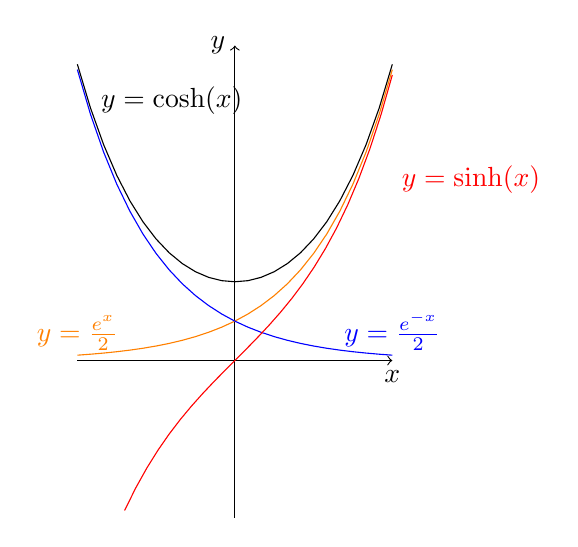
\begin{tikzpicture} 
    	\draw[->] (-2,0) -- (2,0) node[below] {$x$};
    	\draw[->] (0,-2) -- (0,4) node[left] {$y$};
    	\draw[orange, domain= -2:2]  plot (\x, {  exp(\x) * 0.5  } ) ;
    	\draw[orange]  (-2,0) node[above] {$y=\frac{e^ x}{2}$};
    	\draw[ blue, domain= -2:2]  plot (\x, {  exp(-\x) * 0.5  } );
    	\draw[blue]  (2,0) node[above] {$y=\frac{e^ {-x}}{2}$};
    	\draw[red, domain= -1.4:2]  plot (\x, {  exp(\x) * 0.5 -  exp(-\x) * 0.5 } ) ;
    	\draw[red]  (3,2) node[above] {$y=\sinh(x)$};
    	\draw[black, domain= -2:2]  plot (\x, {  exp(\x) * 0.5 +exp(-\x) * 0.5 } );
    	\draw[black]  (-0.8,3) node[above] {$y=\cosh(x)$};
	    \end{tikzpicture} 
	\end{center}
\end{frame}	

\subsection{区域边界条件}
\begin{frame}
	\frametitle{圆域拉普拉斯方程}	
	拉普拉斯算符在不同坐标系中的具体形式\\  \vspace{0.6 cm}	
	直角坐标~ $(x,y,z): $	{ 	$ \displaystyle  \nabla ^{2}  = \frac{\partial ^2}{\partial x^2} +\frac{\partial^2 }{\partial y^2} +\frac{\partial^2  }{\partial z^2}$}\\ 	
	球坐标~ $	(r,\theta, \varphi )$ :
	{ 	$ \displaystyle  \nabla ^{2} =\frac{1}{r^2} \frac{\partial }{\partial r} (r^2\frac{\partial }{\partial r} )+
		\frac{1}{r^2 \sin \theta  } \frac{\partial }{\partial \theta } (\sin \theta \frac{\partial }{\partial \theta } )
		+\frac{1}{r^2 \sin^2 \theta  } \frac{\partial^2}{\partial\varphi ^2}$ } \\ 	
	极坐标~ $	(r,\theta)$ :
	{ 	$ \displaystyle  \nabla ^{2} =\frac{\partial ^2 }{\partial r^2 } +\frac{1}{r } \frac{\partial }{\partial r } +
		\frac{1}{r^2 } \frac{\partial ^2 }{\partial \theta ^2 } $ }\\ 		
\end{frame}	
	
\begin{frame}	
	\begin{exampleblock} {例3、求圆域拉普拉斯方程}
	{ $  \displaystyle  \left \{ 
	\begin{array}{cc}
		\displaystyle {	\frac{\partial^2 u }{\partial r^2 } +\frac{1}{r } \frac{\partial u }{\partial r } +
			\frac{1}{r^2 } \frac{\partial ^2 u }{\partial \theta ^2
		} } =0, ~~ 0<r<r_0\\
		\\
		u(r_0,\theta )=f(\theta ) ,~~~~~~~~~~~~ 0<\theta <2\pi 
	\end{array}
	\right. $}  
	\end{exampleblock}	
	\alert{ 解:}	 
	方程可分离变量,令 $\displaystyle  u(r,\theta)=R(r) \Theta(\theta)$,代回原方程  \\ 
	{ $\displaystyle  R''\Theta +\dfrac{1}{r^2} R\Theta '' +\dfrac{1}{r}R'\Theta=0 $} \\ 
	{ $\displaystyle  \dfrac{r^2R''+rR'}{R}=-\dfrac{\Theta '' }{\Theta} =\lambda $} \\ 
	得两常微分方程:
\end{frame}	

\begin{frame}	
	I、 $\displaystyle 	\Theta '' + \lambda \theta =0 $  \\ 
	定解条件:$\displaystyle 	\Theta(\theta +2 \pi )=\Theta (\theta)  $  \\ 
	II、$\displaystyle  r^2 R'' +r R' -\lambda R =0 $  \\   \vspace{0.6 cm}	
	
	解方程I:  根据以前的分析,在 $\lambda > 0 $ 时,有通解\\ 
	{ $\displaystyle  \Theta(\theta)=A\cos \sqrt{\lambda } \theta+B\sin \sqrt{\lambda }\theta$}\\ 
	由定解条件:$\displaystyle 	\Theta(2 \pi )=\Theta (0)~,~~ 	\Theta' (2 \pi )=\Theta' (0)  $ 得方程: \\ 
	$ \left [
	\begin{array}{lll}
		\cos (\sqrt {\lambda} 2\pi )-1  & \sin (\sqrt {\lambda} 2\pi )\\
		-\sin (\sqrt {\lambda} 2\pi ) & \cos (\sqrt {\lambda} 2\pi )-1
	\end{array} \right] 
	\left [
	\begin{array}{lll}
		A\\
		B
	\end{array} \right] 
	=
	\left [
	\begin{array}{lll}
		0\\
		0
	\end{array} \right]
	$ \\
	系数行列式为零,得\\
	$(\cos (\sqrt {\lambda} 2\pi )-1 ) ^2 + \sin ^2 (\sqrt {\lambda} 2\pi ) =0$ \\ 
\end{frame}	

\begin{frame}
	$\cos (\sqrt {\lambda} 2\pi)=1$   \\ 	
	固有值:$\lambda _n =n^2 ~,~~ (n=0,1,2,...)$  \\ 
	固有函数:$\displaystyle  \Theta(\theta)=A_n\cos n \theta +B_n \sin n \theta $\\   \vspace{0.6cm}

	解方程II:
	{$\displaystyle  r^2 R'' +r R' -\lambda R =0 $  } \\ 
	把$\lambda_n =n^2 $代入, 得 \\ 
	{$\displaystyle  r^2 R'' +r R' -n^2R =0 $  } \\ 
	这是欧拉方程:令 $ r=exp(t) $ ,有 $t=\ln r$, 求导 \\ 
	$ \displaystyle \frac{dR}{dr} =\frac{dR}{dt} \frac{dt}{dr} =\frac{1}{r} \frac{dR}{dt} $ \\ 
	$ \displaystyle \frac{d^2R}{dr^2} =-\frac{1}{r^2}\frac{dR}{dt} + \frac{1}{r} \frac{d}{dr} (\frac{dR}{dt} )$ \\ 
	$ \displaystyle \frac{d^2R}{dr^2} =\frac{1}{r^2} (\frac{d^2R}{dt^2}-\frac{dR}{dt} )$ \\ 		
\end{frame}	

\begin{frame}	
	代回方程,得:\\ 
	$ \displaystyle   \dfrac{d^2R}{dt^2} -n^2 R =0 $ \\ 
	由特征方程有两相异实根,得通解:\\ 
	$ R=C_nexp(nt)+D_n exp(-nt) $\\
	把 $t=\ln r$ 代回,得\\
	$R=C_n r^n +D_nr^{-n}$ \\ 
	第二项发散,应删除,得\\
	$R= C_n r^n,  ~~ (n=0,1,2,......) $		\\
	基本解:\\ 
	$\begin{array}{llll}
		u_n(r,\theta) &=& (a_n\cos n\theta +b_n \sin n \theta ) r^n  \\ 
	\end{array}$ \\ 	
\end{frame}	

\begin{frame}	
	叠加解:\\ 
	$\begin{array}{llll}
		u(r, \theta) &=& \dfrac{1}{2} a_0 +\sum\limits_{n=1}^{\infty } (a_n\cos n\theta +b_n \sin n \theta ) r^n
	\end{array}$ \\ 
	代入定解条件:$ u(r_0,\theta)=f (\theta)   $ \\ 
	$ =  \dfrac{1}{2} a_0 +\sum\limits_{n=1}^{\infty } (a_n\cos n\theta +b_n \sin n \theta ) r_0^n $\\ 
	系数公式:\\ 
	$  \displaystyle  a_n = \dfrac{1}{r_0 ^n \pi }  \int\limits_{0}^{2\pi} f(\theta) \cos n \theta d\theta $ \\ 
	$  \displaystyle  b_n = \dfrac{1}{r_0 ^n \pi }  \int\limits_{0}^{2\pi} f(\theta) \sin n \theta d\theta $  \\ 	
\end{frame}	

\begin{frame}	
	\begin{exampleblock} { 例4、求解如下边值问题}
	{ $  \displaystyle  \left \{ 
	\begin{array}{cc}
		\displaystyle {	\dfrac{\partial^2 u }{\partial r^2 } +\dfrac{1}{r } \dfrac{\partial u }{\partial r } +
		\dfrac{1}{r^2 } \dfrac{\partial ^2 u }{\partial \theta ^2
		} } =0, ~~ 0<r<r_0\\
		\\
		u(r_0,\theta )=A\cos(\theta),~~~~~~~~~ 0<\theta <2\pi 
	\end{array}
	\right. $}  
	\end{exampleblock}	
	\alert{ 解:}	 求系数:\\
	$  \displaystyle  a_1 = \dfrac{1}{r_0 ^1 \pi }  \int\limits_{0}^{2\pi} A\cos(\theta) \cos  \theta d\theta  $ \\ 	
	\hspace{0.8cm}$  \displaystyle  = \dfrac{A}{r_0  \pi }  \int\limits_{0}^{2\pi} \cos ^2 (\theta)  d\theta  = \frac{A}{r_ \pi }  \int\limits_{0}^{2\pi} (1+\cos2\theta) d\theta$ = $\dfrac{A}{r_0}$ \\ 
	$  \displaystyle  a_n = \dfrac{1}{r_0 ^n \pi }  \int\limits_{0}^{2\pi} A\cos(\theta) \cos n \theta d\theta =0~,~ (n\ne 1)$ \\ 
	$  \displaystyle  b_n = \dfrac{1}{r_0 ^n \pi }  \int\limits_{0}^{2\pi} A\cos(\theta) \sin n \theta d\theta =0 $  \\ 
\end{frame}	

\begin{frame}	
	叠加解:\\
	$\begin{array}{llll}
		u(r, \theta) &=& \dfrac{1}{2} a_0 +\sum\limits_{n=1}^{\infty } (a_n\cos n\theta +b_n \sin n \theta ) r^n \\
		&=& \dfrac{1}{2} a_0+ a_1 r\cos \theta \\
		&=&  \dfrac{A}{r_0} r \cos \theta 
	\end{array}$ \\ 
	\begin{block}{Remark}
		若将边界条件修改为: $A \cos 2\theta$ ,或 $A \sin 2\theta $ ,解会如何变化?
	\end{block}
\end{frame}	

\begin{frame}	
%	\frametitle{作业} 
	作业:
	1、求解固有值问题\\ 
	$\begin{array}{lllllllll}
		& \begin{cases}
			Y~^{''} +\lambda Y=0  ~~,~~ 0<y<2\pi \\
			Y(0) =Y(2\pi) , ~~ Y'(0) =Y'(2\pi)
		\end{cases}\\	
	\end{array}$ \\ 
	2、求解圆域边值问题\\
	$\displaystyle  \begin{array}{lllllllll}
	&\begin{cases}
		\dfrac{\partial^2 u }{\partial r^2 } +\dfrac{1}{r } \dfrac{\partial u }{\partial r } +
		\dfrac{1}{r^2 } \dfrac{\partial ^2 u }{\partial \theta ^2  } =0, ~~ 0<r<1\\
		u(1,\theta)= A\cos 2 \theta +B \cos 4 \theta \\	
	\end{cases} \\	
	\end{array}$ \\ 
	3、求解矩形域边值问题\\
	$\begin{array}{lllllllll}
		& \begin{cases}
			u_{xx} +u_{yy} =0 ,~~~~ (0<x, y<1)\\
			u(x,0)= u(0,y)=u(x,1)= 0 \\
			u(1,y)= \sin 2\pi y
		\end{cases}\\	
		&\begin{cases}
			u_{xx} +u_{yy} =0 ,~~~~ (0<x, y<1)\\
			u(1,y)= u(0,y)=u(x,0)= 0 \\
			u(x,1)= \sin n\pi x
		\end{cases} \\	
	\end{array}$ \\ 	
\end{frame}

\begin{frame}
	\frametitle{课外读物和思考}
	了解和学习三大偏微分方程的各种解法:\\
	《Partial Differential Equations》- 作者: Lawrence C. Evans
\end{frame}
%%%%%%%%%%%%%%%%%%%%%%%%%%%%%%			
